\documentclass[12pt, fullpage,letterpaper]{article}

\usepackage[margin=1in]{geometry}
\usepackage{url}
\usepackage{amsmath,amsthm,amssymb}
\usepackage{caption}
\usepackage{subcaption}
\usepackage{float}

\usepackage{pgfplots}
\usepgfplotslibrary{polar}
\usepgflibrary{shapes.geometric}
\usetikzlibrary{calc}

\pgfplotsset{my style/.append style={axis x line=middle, axis y line=
middle, xlabel={$x$}, ylabel={$y$}, axis equal }}

\pdfpageattr {/Group << /S /Transparency /I true /CS /DeviceRGB>>}

\usetikzlibrary{arrows,shapes,positioning}
\usetikzlibrary{decorations.markings}
\tikzstyle arrowstyle=[scale=1]
\tikzstyle directed=[postaction={decorate,decoration={markings,
    mark=at position .65 with {\arrow[arrowstyle]{stealth}}}}]
\tikzstyle reverse directed=[postaction={decorate,decoration={markings,
    mark=at position .65 with {\arrowreversed[arrowstyle]{stealth};}}}]

\newcommand{\semester}{Fall 2015}
\newcommand{\assignmentId}{3}
\newcommand{\releaseDate}{Oct 20, 2015}
\newcommand{\dueDate}{Nov 3, 2015}

\newcommand{\bx}{{\bf x}}
\newcommand{\bw}{{\bf w}}

\title{CS 5350/6350: Machine Learining \semester}
\author{Homework \assignmentId\\ Christopher Mertin}
\date{Handed out: \releaseDate\\
  Due date: \dueDate}

\begin{document}
\maketitle


%\section*{General Instructions}

{\footnotesize
  \begin{itemize}
  \item You are welcome to talk to other members of the class about
    the homework. I am more concerned that you understand the
    underlying concepts. However, you should write down your own
    solution. Please keep the class collaboration policy in mind.

  \item Feel free ask questions about the homework with the instructor
    or the TAs.

  \item Your written solutions should be brief and clear. You need to
    show your work, not just the final answer, but you do \emph{not}
    need to write it in gory detail. Your assignment should be {\bf no
      more than 10 pages}. Every extra page will cost a point.

  \item Handwritten solutions will not be accepted.

  \item The homework is due by midnight of the due date. Please submit
    the homework on Canvas.

  \item Some questions are marked {\bf For 6350 students}. Students
    who are registered for CS 6350 should do these questions. Of
    course, if you are registered for CS 5350, you are welcome to do
    the question too, but you will not get any credit for it.

  \end{itemize}
}

%%% Local Variables:
%%% mode: latex
%%% TeX-master: "hw2"
%%% End:

%\section*{Note}
%Do not just put down an answer. We want an explanation. No points will
%be given for just a statement of the results of a proof. You will be
%graded on your reasoning, not just on your final result. 
%
%Please follow good proof technique; what this means is if you make
%assumptions, state them. If what you do between one step and the next
%is not trivial or obvious, then state how and why you are doing what
%you are doing. A good rule of thumb is if you have to ask yourself
%whether what you're doing is obvious, then it's probably not obvious.
%Try to make the proof clean and easy to follow.

\section{Warm Up: Feature Expansion}
\label{sec:feature-expansion}

[10 points total] Consider an instance space consisting of points on
the two dimensional plane $(x_1,x_2)$. Let $\mathcal{C}$ be a concept
class defined on this instance space. Each function
$f_r \in \mathcal{C}$ is defined by a radius $r$ as follows:
\[
f_r(x_1, x_2) = 
\begin{cases}
  +1  & \text{if } x_1^2 +x_2^2 - 2x_1 \leq r^2 \\
  -1 & \text{else}
\end{cases}
\]
This hypothesis class is definitely not separable in $\mathbb{R}^2$.
That is, there is no $w_1, w_2$ and $b$ such that $f_r(x_1, x_2) =
sign(w_1 x_1 + w_2 x_2 + b)$ for any $r$. 

\begin{enumerate}
\item ~[4 points] Construct a function $\phi(x_1,x_2)$ that maps
  examples to a new space, such that the positive and negative
  examples are linearly separable in that space? That is, after the
  transformation, there is some weight vector $\bw$ and a bias $b$
  such that $f_r(x_1, x_2) = sign(\bw^T\phi(x_1, x_2) + b)$ for any
  value of $r$.

  (Note: This new space need not be a two-dimensional space.)

  \begin{itemize}
    \item The distribution of the postive cases are in a circle that is centered around $(1,0)$. This can be mapped into 3-dimensions by using a Gaussian Distribution over the data. An alternative equation to the problem is $(x-1)^{2}+y^{2}\leq r^{2}+1$ which describes a cirlce of radius $\sqrt{r^{2}+1}$. Then, a plane at $Z=0.1$ (or some other small value for $Z$ to bisect the data) can be used to bisect the data. The formula that would be used is

\[
\phi(x_{1},x_{2}) = \exp\left(-\left(\frac{(x_{1}-1)^{2}}{2\sqrt{r^{2}+1}}\right) + \left(\frac{x_{2}^{2}}{2\sqrt{r^{2}+1}} \right)  \right)
\]

Which will create a Gaussian distribution in the z-dimension for positive examples and wouldn't change anything for the negative examples, which a hyperplane can bisect the two.
  \end{itemize}

\item ~[3 points] If we change the above function to: 
  \[
  g_r(x_1,x_2) = 
  \begin{cases}
    +1 & \text{if } x_1^2 -x_2^2 \leq r^2 \\
    -1 & \text{else}
  \end{cases}
  \]

  Does your $\phi(x_1,x_2)$ make the above linearly separable?  If so
  demonstrate how. If not prove that it does not.

\begin{itemize}
  \item It is trivially seen that $\phi(x_{1},x_{2})$ {\em cannot} make $g_{r}(x_{1},x_{2})$ linearlly separable as $\phi$ was a gaussian distribution in the shape of a cirlce. This allowed to raise the positive points above the axis. $g_{r}$ is a hyperbola, and therefore cannot be linarly separated by a gaussian distribution.
\end{itemize}

\item ~[3 points] Does $\phi(x_1,x_2) = [x_1,x_2^2]$ make the function
  $g_r$ above linearly separable? If so demonstrate how. If not prove
  that it does not.

\begin{itemize}
\item This can be shown graphically that this is {\em not} the case for all $r$. By taking the plots and plotting them in the $3^{rd}$ dimension, it can be trivially seen that there is no segment/hyper plane that can be drawn through the data. Figure~\ref{fig:3Dplot} shows the plot of $x^{2}-y^{2}\leq 2^{2}$, while Figure~\ref{fig:Contourplot} is of taking the data points in Figure~\ref{fig:3Dplot} and squaring the $y$ value, while keeping the classificataions.

%\item This can be shown graphically that it is the case. By taking the plots and plotting them in a higher $3^{rd}$ dimension, it can be trivally seen that there is a segment/hyper plane that can be drawn through the data. Figure~\ref{fig:3Dplot} shows the function plotted in 3 dimensions while Figure~\ref{fig:Contourplot} makes the bisection point easier to see by plotting it in two dimensions.

\begin{figure}
\centering
\begin{minipage}{.5\textwidth}
  \centering
  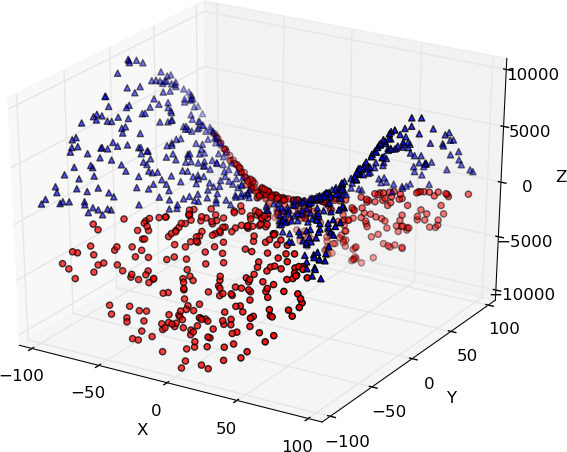
\includegraphics[width=\linewidth]{normal-1000-3.png}
  \captionof{figure}{Plot of $x^{2}-y^{2}\leq 2^{2}$}
  \label{fig:3Dplot}
\end{minipage}%
\begin{minipage}{.5\textwidth}
  \centering
  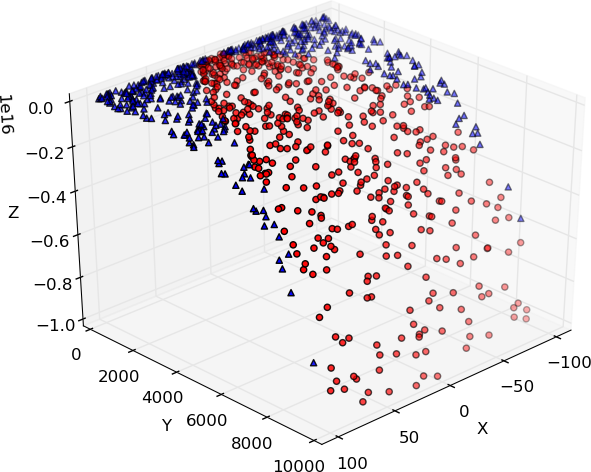
\includegraphics[width=\linewidth]{phi-1000-3.png}
  \captionof{figure}{Plot of $\phi(x,y)$}
  \label{fig:Contourplot}
\end{minipage}
\end{figure}
\end{itemize}

\end{enumerate}


%%% Local Variables:
%%% mode: latex
%%% TeX-master: "hw3"
%%% End:


\section{PAC Learning}
\label{sec:pac-learning}
\begin{enumerate}

\item ~[15 points] Due to the recent budget cuts the government no
  longer has any money to pay for humans to monitor the state of
  nuclear reactors. They have charged you with assessing a Robot's
  ability to perform this vital task. Every reactor has a different
  number of binary gauges which indicate whether or not some aspect of
  the reaction is {\tt normal} or {\tt strange}. The reactor itself
  can be in one of {\bf five} states -- {\em Normal}, {\em Meltdown},
  {\em Pre-meltdown}, {\em Abnormally cool} or {\em Off}. Each
  combination of the binary guage settings indicate one of these five
  reactor states. We want to know if we can train a robot to identify
  which gauges and gauge combinations are responsible for each reactor
  state.

  \begin{enumerate}
  \item [a)][5 points] Suppose that we have $N$ gauges with which to
    identify reactor states. How large is the hypothesis space for
    this task? (You may have to make assumptions about the underlying
    function space. State your assumptions clearly.)

\begin{itemize}
  \item We can {\em assume} that since this is a nuclear reactor that all of the gauges are important, and thus there are $3^{N}$ different conjunctions for determining the state of the nuclear reactor.%Where $K$ is the number of gauges that need to be looked at, we can say there is a hypothesis space of ${N \choose K}$. For this to be true, we have to assume that there are no repetitions. Or, we can {\em assume} that since this is a nuclear reactor, all of the gauges are important so there is $3^{N}$ different conjunctions for determining the states.
\end{itemize}

  \item[b)] [10 points] The ex-government employee, whose job the
    robot is taking, trains the robot at a nuclear reactor where there
    are 20 gauges by showing the robot a set of gauge positions for
    the five different reactor states. If the robot wants to learn to
    recognize the reactor's condition with .1 percent error with
    greater than 99\% probability how many examples does the robot
    need to see?
\begin{itemize}
\item The following equation represents the relation for PAC learning
\begin{align*}
\delta &\geq He^{-\epsilon R}\\
\intertext{Where $R$ is the number of required training examples, $\epsilon$ is the error, and $\delta$ is the probability. We can solve for $R$ to get the maximum number of training examples.}
\frac{1}{\epsilon}\log\left( {\frac{\delta}{H}}\right) &\geq -R\\
\frac{1}{\epsilon}\log\left( {\frac{H}{\delta}}\right) &\geq R\\
\frac{1}{\epsilon}\left[n\log(3) - \log(\delta) \right] &\geq R\\
\intertext{where $\delta$ is defined as $(1-\text{probability})$ and $\epsilon$ is defined as $(1-\text{accuracy})$. We can plug these in from the stated problem and we get}
\frac{1}{0.10}\left(20\log(3) - \log(0.01) \right) &\geq R\\
R &\leq 266
\end{align*}
\end{itemize}

  \end{enumerate}


\item ~[5 points] Is it possible for a learned hypothesis $h$ to
   achieve 100\% accuracy with respect to a training set and still
   have non-zero true error? If so, provide a description of how this
   is possible. If not, prove that it is impossible.

\begin{itemize}
\item Yes, an instance of this would be when the data is overfit to the training data, which would result in 100\% accuracy on the training set and a large (non-zero) error on the test set, which would result in a non-zero true error.
\end{itemize}


\item ~[25 points] {\bf Learning decision lists:}
  In this problem, we are going to learn the class of $k$-decision
lists. A decision list is an ordered sequence of if-then-else
statements. The sequence of if-then-else conditions are tested in
order, and the answer associated to the first satisfied condition is
output. See Figure~\ref{fig:decision_list} for an example of a
$2$-decision list.

\begin{figure}[!h]
\begin{center}
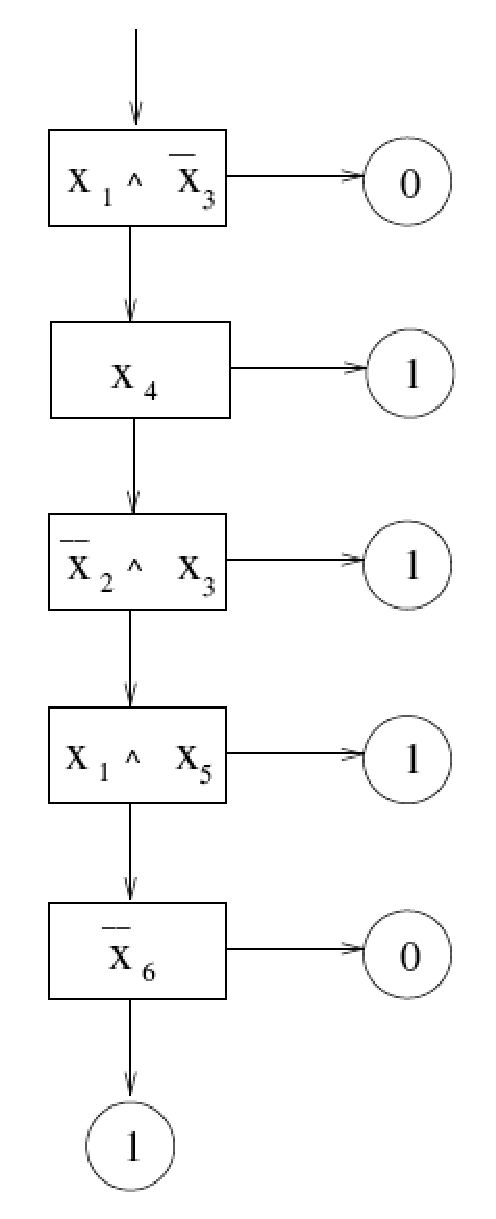
\includegraphics[width=1.35in]{fig-1.pdf}
\caption{A $2$-decision list.}
\label{fig:decision_list}
\end{center}
\end{figure}

A {\em $k$-decision list} over the variables $x_{1}, \ldots, x_{n}$ is
an ordered sequence $L=(c_{1}, b_{1}), \ldots, (c_{\ell},b_{\ell})$ and a
bit $b$, in which each $c_{i}$ is a conjunction of at most $k$
literals over $x_{1},\ldots, x_{n}$. The bit $b$ is called the {\em
  default} value, and $b_{i}$ is referred to as the bit {\em
  associated} with condition $c_{i}$. For any input $x \in \{0,
1\}^{n}$, $L(x)$ is defined to be the bit $b_{j}$, where $j$ is the
smallest index satisfying $c_{j}(x)=1$; if no such index exists, then
$L(x)=b$.

We denote by $k\mbox{\em -DL}$ the class of concepts that can be
represented by a $k$-decision list.


\begin{enumerate}
\item \relax[8 points] Show that if a concept $c$ can be represented
  as a $k$-decision list so can its complement, $\neg c$. You can show
  this by providing a $k$-decision list that represents $\neg c$,
  given $c = \{(c_{1},b_{1}), \ldots, (c_{\ell},b_{\ell}),b\}$.

\begin{itemize}
\item To prove that the complement of $c$ is a $k$-decision list, we can simply take $c$ and negate all of the bits to produce another $k$-decision list. It would look such as the following: $\neg c = \{(c_{1},\neg b_{1}), \ldots, (c_{\ell},\neg b_{\ell}),\neg b\}$, which is a $k$-decision list.
\end{itemize}
\item \relax[9 points] Use  Occam's Razor to show: \\
  For any constant $k \geq 1$, the class of $k$-decision lists is
  PAC-learnable.

\begin{itemize}
\item Occam's Razor states that the least complicated case is most likely true, but in this course we take it as being true. Therefore, we can show this to be PAC-learnable by finding a lower bound on the set such that it is the minimum $k$-decision list. This can be done by showing that the dimensions of data needed is {\em finite}.

It can be trivially seen that the size of the concept class is $\left| c_{k} \right| = \mathcal{O}\left( n^{k}\right)$. Each of the bits belong in $b_{i}\in \{ 0,1 \}$, and since there are $\ell$ of them it results in $2^{\ell}$ different combinations. There are also $\ell!$ orderings of those bits. Finally, the size of the concept class that can describe the data is $2^{\left| c_{k} \right|}$. Therefore, the overall bound is represented by the product of these three which is $\mathcal{O}\left( 2^{\left| c_{k} \right|}\cdot \ell!\cdot 2^{\ell} \right)$. However, the {\em maximum value} of $\ell$ is represented by $\left| c_{k} \right|$, so we can simplify our notation as $\mathcal{O}\left( 2^{2\left| c_{k}\right|}\left| c_{k} \right|!\right)$.

Finally, the size of the number of examples needed in our set is logarithmically proportional to the size of the concept class, so by taking the log we get $\mathcal{O}\left( 2n^{k}\log(2) + kn^{k}\log(n)\right)$ which is a {\em finite number} for any $k\geq 1$ and thus is PAC-learnable.
\end{itemize}
\item \relax[8 points] Show that $1$-decision lists are a linearly
  separable functions. (Hint: Find a weight vector that will make the
  same predictions a given $1$-decision list.)

\begin{itemize}
\item To do this, we need to construct our $\mathbf{x}$ vector and then our $\mathbf{w}$ vector where $\mathbf{w}$ is the weight vector defined as $\mathbf{w} = (\theta , w_{1}, w_{2}, \ldots , w_{\ell})^{T}$ with $\theta$ being the bias. We can define our $\mathbf{x}$ vector as $\mathbf{x} = (1, x_{1}, x_{2}, \ldots, x_{\ell})^{T}$ with the leading term being needed to support the bias. $x_{i}$ can be defined by the value of $b_{i}$, where $x_{i} = -1$ for $b_{i} = 0$, and $x_{i} = 1$ for $b_{i} = 1$. From here, we can create a threshold function to ``learn'' the $k$-decision list, which is defined as $\mathbf{w}^{T}\cdot \mathbf{x} \geq 0$.

In building $\mathbf{w}$, we can define each element of $w_{i} = b_{i}\cdot 2^{\ell+1-i}$ as to separate the individual data points. This would make the first few elements $\mathcal{O}\left(\pm 2^{\ell}\right)$ and the last elements $\mathcal{O}(\pm 2)$, where the $\pm$ comes about due to the individual bit $b_{i}$. Following this, we can look at the original 1-DL and if the overall/default bit is false, then we can set $\theta = -1$, else $\theta = 1$. This would overall be equivalent to the 1-DL and would make it liearly separable and learnable.
\end{itemize}
\end{enumerate}



%%% Local Variables: 
%%% mode: latex
%%% TeX-master: "hw3"
%%% End: 


\item ~[20 points, {\bf CS 6350 students only}] Let $X$ be an instance
  space and let $D_1,D_2,...,D_m$ be a sequence of distributions over
  $X$. Let $\mathcal{H}$ be a finite class of binary classifiers over
  $X$ and let $f\in \mathcal{H}$. 

  Suppose we have a sample $S$ of $m$ examples, such that the
  instances are independent but are not identically distributed. The
  $i^{th}$ instance is sampled from $D_i$ and then $y_i$ is set to be
  $f(x_i)$. Let $\bar{D}_m$ denote the average, that is,
  $\bar{D}_m = \frac{1}{m}\sum_{i=1}^m D_i$. 

  Let $h \in \mathcal{H}$ be a classifier that gets zero error on the
  training set. That is, for every example $x_i \in X$, we have
  $h(x_i) = f(x_i)$. Show that, for any accuracy parameter
  $\epsilon \in (0, 1)$, the probability that the expected error of
  the learned classifier $h$ is greater than $\epsilon$ is no more
  than $|\mathcal{H}|e^{-\epsilon m}$. That is, show that

  \[\mathbb{P}\left[E_{x \sim \bar{D}_m}\left[h(x) \ne f(x)\right]> \epsilon\right] \leq  |\mathcal{H}|e^{-\epsilon m}\]

  (Hint: You have to use the fact that the arithmetic mean of a set of
  non-negative numbers greater than or equal to their geometric mean.)

\begin{itemize}
\item We can say that the expection value of the function is defined as
\begin{align*}
E_{x \sim \bar{D}_m}(\mathbb{I}_{\{h(x) = f(x)\}}) &= E_{x\sim \bar{D}_m}(\mathbb{Z}(x))\\
\intertext{Where the second relation is the same but $\mathbb{Z}(x)$ was introduced to shorten notation. We can say that this relation is equivalent to}
E_{x\sim \bar{D}_m}(\mathbb{Z}(x)) &= \underbrace{\sum_{x}\bar{D}(x)}_{\frac{1}{m}\sum_{i=1}^{m}D_{i}(x)}\mathbb{Z}(x) = \frac{1}{m}\sum_{x}\sum_{i=1}^{m}D_{i}(x)\mathbb{Z}(x)
\intertext{From here, we can switch the summations}
&= \frac{1}{m}\sum_{i=1}^{m}\underbrace{\sum_{x}D_{i}(x)\mathbb{Z}(x)}_{E_{x\sim D_{i}}} = \frac{1}{m}\sum E_{x\sim D_{i}}\mathbb{Z}(x)\quad (1)\\
\intertext{From the above problem, we can see that it's an independent distribution of probabilities, though it is not uniform. Therefore, we have the total probability as being}
P\left( \mathbb{Z}(x_{i})\ \forall i\right) &= \prod_{i=1}^{m}P\left( \mathbb{Z}(x_{i}) \right) \leq \left( \frac{1}{m}\sum_{i=1}^{m}P\left( \mathbb{Z}(x_{i})\right) \right)^{m} \quad (2)
\intertext{Where $(2)$ comes about because $\frac{1}{m}\sum_{i=1}^{m}x_{i} \geq \left( \prod_{i=1}^{m}x_{i} \right)^{\frac{1}{m}}$. By plugging $(1)$ into $(2)$, we get}
&= \left( \frac{1}{m}\sum_{i=1}^{m}E_{x\sim D_{i}}\left[ \mathbb{Z}(x)\right] \right)^{m} < (1-\epsilon)^{m}\\
\intertext{From here we can say that $(1-x) < e^{-x}$ as $(1-x)$ is a first order taylor series expansion of $e^{-x}$. Therefore, we reduce it to the following relation}
 &< e^{-m\epsilon}\\
\intertext{Where we can then apply the {\em Union Bound}, which states that the probability of at least one event happening is less than the sum of the probabilities of the individual events.}
&< \left| H \right|e^{-m\epsilon}
\end{align*}
\end{itemize}
\end{enumerate}

%%% Local Variables:
%%% mode: latex
%%% TeX-master: "hw3"
%%% End:


\section{VC Dimension}
\label{sec:vc-dimension}
\begin{enumerate}
\item ~[5 points] Assume that the three points below can be labeled
  in any way.  Show with pictures how they can be shattered by a
  linear classifier.  Use filled dots to represent positive classes
  and unfilled dots to represent negative classes.


  \begin{tikzpicture}
    \begin{axis}[my style, xtick={-1,0,...,3}, ytick={-1,0,...,3},
      xmin=-1, xmax=3, ymin=-1, ymax=3]
      \addplot[mark=*,only marks] coordinates {(2,2)(1,1)(1,2)};
    \end{axis}
  \end{tikzpicture}

%%%%%%%%%%%%%%% 1st set
  \begin{tikzpicture}
    \begin{axis}[my style, xtick={-1,0,...,3}, ytick={-1,0,...,3},
      xmin=-1, xmax=3, ymin=-1, ymax=3]
      \addplot[mark=o,only marks] coordinates {(1,1)};
      \addplot[mark=*,only marks] coordinates {(1,2)};
      \addplot[mark=*,only marks] coordinates {(2,2)};
      \draw [draw=red, dashed, ultra thick] (axis cs: -1,1.5) -- (axis cs: 3,1.5);
      %\draw [->, draw=red, ultra thick] (axis cs: 1.5,1.5) -- (axis cs: 1.5, 2);
    \end{axis}
  \end{tikzpicture}
  \begin{tikzpicture}
    \begin{axis}[my style, xtick={-1,0,...,3}, ytick={-1,0,...,3},
      xmin=-1, xmax=3, ymin=-1, ymax=3]
      \addplot[mark=*,only marks] coordinates {(1,1)};
      \addplot[mark=o,only marks] coordinates {(1,2)};
      \addplot[mark=*,only marks] coordinates {(2,2)};
      \draw [draw=red, dashed, ultra thick] (axis cs: -.75,0.5) -- (axis cs: 3,3);
      %\draw [->, draw=red, ultra thick] (axis cs: 1.35,1.75) -- (axis cs: 1.5, 1.5);
    \end{axis}
  \end{tikzpicture}

%%%%%%%%%%%%%%% 2nd set
  \begin{tikzpicture}
    \begin{axis}[my style, xtick={-1,0,...,3}, ytick={-1,0,...,3},
      xmin=-1, xmax=3, ymin=-1, ymax=3]
      \addplot[mark=*,only marks] coordinates {(1,1)};
      \addplot[mark=*,only marks] coordinates {(1,2)};
      \addplot[mark=o,only marks] coordinates {(2,2)};
      \draw [draw=red, dashed, ultra thick] (axis cs: 1.5,-1) -- (axis cs: 1.5,3);
      %\draw [->, draw=red, ultra thick] (axis cs: 1.5,1.5) -- (axis cs: 1.5, 2);
    \end{axis}
  \end{tikzpicture}
 \begin{tikzpicture}
    \begin{axis}[my style, xtick={-1,0,...,3}, ytick={-1,0,...,3},
      xmin=-1, xmax=3, ymin=-1, ymax=3]
      \addplot[mark=*,only marks] coordinates {(1,1)};
      \addplot[mark=o,only marks] coordinates {(1,2)};
      \addplot[mark=o,only marks] coordinates {(2,2)};
      \draw [draw=red, dashed, ultra thick] (axis cs: -1,1.5) -- (axis cs: 3,1.5);
      %\draw [->, draw=red, ultra thick] (axis cs: 1.5,1.5) -- (axis cs: 1.5, 2);
    \end{axis}
  \end{tikzpicture}

%%%%%%%%%%%%%%% 3rd set
  \begin{tikzpicture}
    \begin{axis}[my style, xtick={-1,0,...,3}, ytick={-1,0,...,3},
      xmin=-1, xmax=3, ymin=-1, ymax=3]
      \addplot[mark=o,only marks] coordinates {(1,1)};
      \addplot[mark=o,only marks] coordinates {(1,2)};
      \addplot[mark=*,only marks] coordinates {(2,2)};
      \draw [draw=red, dashed, ultra thick] (axis cs: 1.5,-1) -- (axis cs: 1.5,3);
      %\draw [->, draw=red, ultra thick] (axis cs: 1.5,1.5) -- (axis cs: 1.5, 2);
    \end{axis}
  \end{tikzpicture}
\begin{tikzpicture}
    \begin{axis}[my style, xtick={-1,0,...,3}, ytick={-1,0,...,3},
      xmin=-1, xmax=3, ymin=-1, ymax=3]
      \addplot[mark=o,only marks] coordinates {(1,1)};
      \addplot[mark=*,only marks] coordinates {(1,2)};
      \addplot[mark=o,only marks] coordinates {(2,2)};
      \draw [draw=red, dashed, ultra thick] (axis cs: -.75,0.5) -- (axis cs: 3,3);
      %\draw [->, draw=red, ultra thick] (axis cs: 1.35,1.75) -- (axis cs: 1.5, 1.5);
    \end{axis}
  \end{tikzpicture}

%%%%%%%%%%%%%%% 4th set
  \begin{tikzpicture}
    \begin{axis}[my style, xtick={-1,0,...,3}, ytick={-1,0,...,3},
      xmin=-1, xmax=3, ymin=-1, ymax=3]
      \addplot[mark=*,only marks] coordinates {(1,1)};
      \addplot[mark=*,only marks] coordinates {(1,2)};
      \addplot[mark=*,only marks] coordinates {(2,2)};
      \draw [draw=red, dashed, ultra thick] (axis cs: -1,-1) -- (axis cs: 3,2);
      %\draw [->, draw=red, ultra thick] (axis cs: 1.5,1.5) -- (axis cs: 1.5, 2);
    \end{axis}
  \end{tikzpicture}
\begin{tikzpicture}
    \begin{axis}[my style, xtick={-1,0,...,3}, ytick={-1,0,...,3},
      xmin=-1, xmax=3, ymin=-1, ymax=3]
      \addplot[mark=o,only marks] coordinates {(1,1)};
      \addplot[mark=o,only marks] coordinates {(1,2)};
      \addplot[mark=o,only marks] coordinates {(2,2)};
       \draw [draw=red, dashed, ultra thick] (axis cs: -1,-1) -- (axis cs: 3,2);
      %\draw [->, draw=red, ultra thick] (axis cs: 1.35,1.75) -- (axis cs: 1.5, 1.5);
    \end{axis}
  \end{tikzpicture}

  
\item {\bf VC-dimension of axis aligned rectangles in $\mathbb{R}^d$}:
  Let $H^d_{rec}$ be the class of axis-aligned rectangles in
  $\mathbb{R}^d$. When $d=2$, this class simply consists of rectangles
  on the plane, and labels all points strictly outside the rectangle
  as negative and all points on or inside the rectangle as positive.
  In higher dimensions, this generalizes to $d$-dimensional boxes,
  with points outside the box labeled negative.

  \begin{enumerate}
  \item ~[10 points] Show that the VC dimension of $H^2_{rec}$ is 4.

\begin{tikzpicture}
    \begin{axis}[my style, xtick={-1,0,...,3}, ytick={-1,0,...,3},
      xmin=-1, xmax=3, ymin=-1, ymax=3]
      \addplot[mark=*,only marks] coordinates {(.2,1.8)};
      \addplot[mark=*,only marks] coordinates {(2.8,.2)};
      \addplot[mark=o,only marks] coordinates {(3.2,1)};
      \addplot[mark=o,only marks] coordinates {(1.5,2.2)};	
       \draw [draw=blue, dashed, ultra thick] (axis cs: 0,0) -- (axis cs: 0,2);
       \draw [draw=blue, dashed, ultra thick] (axis cs: 0,2) -- (axis cs: 3,2);
       \draw [draw=blue, dashed, ultra thick] (axis cs: 3,2) -- (axis cs: 3,0);
      \draw [draw=blue, dashed, ultra thick] (axis cs: 3,0) -- (axis cs: 0,0);
      %\draw [->, draw=red, ultra thick] (axis cs: 1.35,1.75) -- (axis cs: 1.5, 1.5);
    \end{axis}
  \end{tikzpicture}

\begin{itemize}
\item Need 4 because we need to define the outer regions of the box. Since the box is axis-aligned, that means that two of the sides are already defined so we need to restrict them such that the other two are as well. We then need to define the {\em inside} of the box by having {\em at least} two points to define the max. 5 points in this instance cannot be shattered. 
\end{itemize}


  \item ~[10 points] Generalize your argument from the previous proof
    to show that for $d$ dimensions, the VC dimension of $H^d_{rec}$
    is $2d$.
\begin{itemize}
\item To generalize the logic in the above step, each dimension needs at least 2 points so that a line can shatter them. In the previous example, the blue line on the right shatters the points $(2.8,0.2)$ and $(3.2,1.0)$, as does the line for the other two points. Therefore, for the line to shatter the points, there must be two in each dimension. It is only restrictecd to 2 because the box is axis-aligned meaning that two of the lines run along the axis of the box and are therefore already defined.
\end{itemize}
  \end{enumerate}
  
\item In the lectures, we considered the VC dimensions of infinite
  concept classes. However, the same argument can be applied to finite
  concept classes too. In this question, we will explore this setting.

  \begin{enumerate}
  \item ~[10 points] Show that for a finite hypothesis class
    $\mathcal{C}$, its VC dimension can be at most
    $\log_2\left(|\mathcal{C}|\right)$. (Hint: You can use
    contradiction for this proof. But not necessarily!)

\begin{itemize}
\item First, we can assume that $VC(\left|\mathcal{C}\right|)=d$, where $d$ is the number of dimensions and $\left|\mathcal{C} \right|$ is the size of the hypothesis class. From here, we can come to the conclusion that there are $2^{d}$ {\em unique} hypotheses in the hypothosis space in order to shatter $d$ instances. Therefore, we have the following

\begin{align*}
2^{d} &\leq \left| \mathcal{C}\right|\\
d\log_{2}(2) &\leq \log_{2}(\left| \mathcal{C}\right|)\\
VC(\left| \mathcal{C}\right|) = d &\leq \log_{2}(\left| \mathcal{C}\right| )
\end{align*}

Where the last relation comes about since $VC(\left| \mathcal{C}\right|) = d$.
\end{itemize}
  \item ~[5 points] Find an example of a class $\mathcal{C}$ of
    functions over the real interval $X = [0,1]$ such that
    $\mathcal{C}$ is an {\bf infinite} set, while its VC dimension is
    exactly one.

\begin{tikzpicture}
\node at (4.15,-.25) {$a$};

    \begin{axis}[my style, xtick={0,1}, ytick={0,.5,1,1.5,2},
      xmin=0, xmax=1, ymin=-0, ymax=2]
\draw[fill=red,opacity=.7]
    (axis cs:0,0) -- (axis cs:0,1.75) -- (axis cs:.75,1.75) -- (axis cs:.75,0) -- cycle ;
\draw[fill=blue,opacity=.7]
    (axis cs:.75,0) -- (axis cs:.75,1.75) -- (axis cs:1,1.75) -- (axis cs:1,0) -- cycle ;
      %\draw [->, draw=red, ultra thick] (axis cs: 1.35,1.75) -- (axis cs: 1.5, 1.5);
    \end{axis}
  \end{tikzpicture}

\begin{itemize}
\item Such that the dividing line is at some point $(0,a)$ and $(a,1)$ where one region is marked as positive and the other as negative. By confining the points to these two regions, there are an infinite number of points in each region but they can be classified by a single line.
\end{itemize}
  \item ~[5 points] Give an example of a {\bf finite} class
    $\mathcal{C}$ of functions over the same domain $X = [0,1]$ whose
    VC dimension is exactly $\log_2(|\mathcal{C}|)$.

\begin{itemize}
\item We can use the example from question 1 of this section as a case. If you have $N$ literals then you will have a concept class size of $2^{N}$, which would have a VC-dimension of $N$ if you take the size to be $\log_{2}\left( 2^{N}\right)$.
\end{itemize}

  \end{enumerate}
  
\end{enumerate}

%%% Local Variables:
%%% mode: latex
%%% TeX-master: "hw3"
%%% End:



\end{document}
%%% Local Variables:
%%% mode: latex
%%% TeX-master: t
%%% End:
